%% This is file `sample-sigconf.tex',
%% generated with the docstrip utility.
%%
%% The original source files were:
%%
%% samples.dtx  (with options: `sigconf')
% TODO: Change to review before submitting
\documentclass[sigconf]{acmart}
%% \BibTeX command to typeset BibTeX logo in the docs
\AtBeginDocument{%
  \providecommand\BibTeX{{%
    \normalfont B\kern-0.5em{\scshape i\kern-0.25em b}\kern-0.8em\TeX}}}

%% Rights management information.  This information is sent to you
%% when you complete the rights form.  These commands have SAMPLE
%% values in them; it is your responsibility as an author to replace
%% the commands and values with those provided to you when you
%% complete the rights form.
\setcopyright{acmcopyright}
\copyrightyear{2024}
\acmYear{2024}
\acmDOI{XXXXXXX.XXXXXXX}

\acmConference[ICSE 2024]{46th International Conference on Software Engineering}{April 2024}{Lisbon, Portugal}

% My packages
\usepackage[nameinlink]{cleveref} % Reference footnotes.
% My packages end

%%
%% end of the preamble, start of the body of the document source.
\begin{document}

%%
%% The "title" command has an optional parameter,
%% allowing the author to define a "short title" to be used in page headers.
\title{Implementing the Visual Debugger: Past, Present, and Future}
% Alternative titles
% Implementing the Visual Debugger: Past, Present, and Future
% Implementing the Visual Debugger: Past, An experience report
% Something regarding IDE integration?

\author{Tim Kr\"{a}uter}
\email{tkra@hvl.no}
\orcid{0000-0003-1795-0611}
\affiliation{%
  \institution{Western Norway University of Applied Sciences}
  \city{Bergen}
  \country{Norway}
}

\author{Adrian Rutle}
\email{aru@hvl.no}
\orcid{0000-0002-4158-1644}
\affiliation{%
  \institution{Western Norway University of Applied Sciences}
  \city{Bergen}
  \country{Norway}
}

\author{Harald K\"{o}nig}
\email{harald.koenig@fhdw.de}
\orcid{0000-0001-6304-6311}
\affiliation{%
  \institution{University of Applied Sciences, FHDW}
  \city{Hannover}
  \country{Germany}}
\affiliation{%
  \institution{Western Norway University of Applied Sciences}
  \city{Bergen}
  \country{Norway}
}

\author{Yngve Lamo}
\email{yla@hvl.no}
\orcid{0000-0001-9196-1779}
\affiliation{%
  \institution{Western Norway University of Applied Sciences}
  \city{Bergen}
  \country{Norway}
}

% \author{Patrick Stünkel \orcidlink{0000-0002-0537-295X}}
% \email{patrick.stuenkel@hvl.no}
% \orcid{0000-0002-0537-295X}
% \affiliation{%
%   \institution{Western Norway University of Applied Sciences}
%   \city{Bergen}
%   \country{Norway}
% }

\renewcommand{\shortauthors}{Kräuter et al.}
\newcommand{\intellij}{IntelliJ IDEA } % <-- Space has to be there
% Four pages + 1 page of references.

%%
%% The abstract is a short summary of the work to be presented in the
%% article.
\begin{abstract}
  TODO: Abstract
A demonstration of the visual debugger is available at \url{https://www.youtube.com/watch?v=lU_OgotweRk}.
\end{abstract}

\keywords{IDE integration, Plugin, Debugging, Visual Debugging, Experience Report}

% Fitting topics from the workshop:
% 1. The development of plugins, add-ons, and extensions for IDEs.
% 2. Visualizations in the IDEs.
% 3. Anecdotal experience about why a certain tool or research approach was not implemented on top of the IDE infrastructure but researchers chose alternatives (e.g., a CLI tool), what the blockers were, and how the IDEs can improve to become more convenient for prototyping.

\received{7 December 2023}
% \received[revised]{7 December 2023}
% \received[accepted]{11 January 2024}

\maketitle

\section{Introduction}
% Context about the tool --> More high level do not repeat too much regarding section 2.
This paper details the experience of implementing the visual debugger \cite{krauterVisualDebuggerTool2022}.
The tool is available for \intellij and Android studio as a plugin \cite{timkrauterVisualDebuggerIntelliJ2023}, but its architecture makes it easily adaptable to other Integrated Development Environments (IDEs) \cite{krauterVisualDebuggerTool2022}.

% Motivation for this report?
% Roadblocks hampering full IDE integration: Swing, Tradeoff tight integration and reusability
% Open problems due to IDE integration: Performance?

% Paper outline
The remainder of this paper is structured as follows.
We describe the visual debugger tool in detail (\cref{sec:visualDebugger}) and outline the lessons we learned and roadblocks we encountered in \cref{sec:lessonsLearned}.
Finally, we discuss related work in \cref{sec:relatedWork} and conclude in \cref{sec:conclusion}.


\section{The Visual Debugger} \label{sec:visualDebugger}
% What can the tool do?
The Visual Debugger is an open-source \intellij plugin that visualizes the debugging variables as an object diagram to foster program comprehension.
It is available for \intellij and Android Studio through the JetBrains Marketplace \cite{timkrauterVisualDebuggerIntelliJ2023, timkrauterVisualDebuggerTool2023}.
% Motivation
Debugging information might not present in the top-level variables and has to be obtained by digging multiple levels (following links to related objects) deep into different variables.
Thus, in specific scenarios, especially when data is hierarchically structured, a graphical representation results in faster and better understanding of the debugging information \cite{krauterVisualDebuggerTool2022}.

% How does the tool work. Give an example
\subsection{Example}

\subsection{Design Principles}
% Inspired by https://github.com/bpmn-io/design-principles
% Take-aways, key design principles/goals
% Straight forward
Using the the Visual debugger is \textit{straightforward} since it becomes automatically available during debugging in the IDE.
% Familiar
Similar to the traditional textual debugging it allows interactions to explore debugging variables in more detail.
% Non-intrusive
In addition, it is \textit{non-intrusive} since it can be used alongside the traditional textual debugging available in the IDE.
% Minimalistic: Less is more


\subsection{Architecture}
% How does the tool achieve this? Architecture and details.

\begin{figure}[ht]
  \centering
  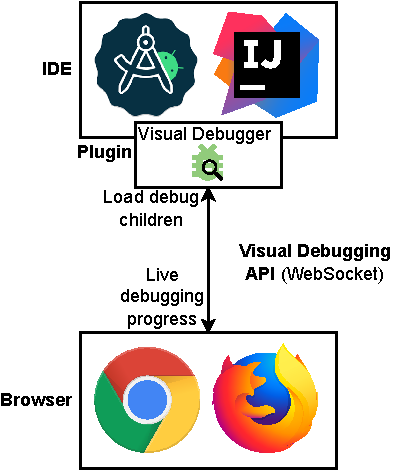
\includegraphics[width=0.7\linewidth]{images/visual-debugger.pdf}
  \caption{Visual Debugger Architecture}
\end{figure}
% Hooks seamlessly into the IntelliJ debugging process using provided APIs.
% has a debugger integrated into the tool, which is not the interactive and interactive one using the WebSocket connection shown in the architecture. Why two is described later maybe teased here: I don't want to use Swing. Swing tools like yfiles are expensive and unsuitable for "free, open-source plugins" <-- check this claim.

% Feedback for the tool and current vs previous downloads.
So far, we have received only positive feedback regarding the visual debugger, and it was downloaded nearly 6600 times \footnote{Last checked on the 26th of October, 2023, see \cite{timkrauterVisualDebuggerIntelliJ2023}.}.
Our tool's downloads doubled compared to the roughly 2700 downloads on the 21st of Juli, 2022, when we published our research paper \cite{krauterVisualDebuggerTool2022} about the visual debugger.

\section{Lessons Learned \& Roadblocks} \label{sec:lessonsLearned}

% Roadblock: Missing APIS
% \subsection{IDE APIs}
% Go plugin not possible due to lacking APIs? --> Access to the APIs needed to integrate plugins with the IDE deeply. Deeper integration means less portability (to other ides) but a better user experience.
% Or it is possible but the integration would not be nice! Since now two people connect to the same process or something similar?

% \section{Improvements to the Visual Debugger}
% Going back in time, i.e., showing previous debugging states. Show class/file and line information somewhere in the UI.
% Highlighting changes.
% Smarter UI. Shows if more information is available (colors and icons). --> Colors and overlays can be adapted from BPMN-js


\section{Related work} \label{sec:relatedWork}

\section{Conclusion} \label{sec:conclusion}

Object diagram modeler: \cite{timkrauterObjectDiagramModeler2023}

% \section{Acknowledgments}

\bibliographystyle{ACM-Reference-Format}
\bibliography{bib}
\end{document}
